\section{Model d'operacions}

En aquesta secció es defineixen els operadors que permeten modelar el
comportament i la manipulació de les dades en el model de \gls{SGSTM}.

Per a treballar amb les sèries temporals multiresolució s'utilitzen
els conceptes descrits al model d'operacions de \gls{SGST}. El model de
\gls{SGSTM} es defineix a partir del model de \gls{SGST} i per tant les operacions
dels \gls{SGSTM} també hi estan basades. Tot i així cal tenir en compte dues
particularitats.

Per una banda, el model de \gls{SGSTM} té una estructura específica que
requereix ser manipulada coherentment. Així, es defineixen operadors
que saben treballar amb aquesta estructura agrupats en dos grups.  El
primer grup són els operadors requerits pel model estructural;
operadors que són inseparables de l'estructura i són utilitzats en el
procés d'emmagatzemar les mesures. El segon grup són els operadors
necessaris per a manipular l'estructura; és a dir operadors que
permeten fer canvis en l'esquema de la base de dades o consultar
paràmetres de l'esquema actual.

Per altra banda, el model de \gls{SGSTM} treballa amb sèries temporals
multiresolució. Així, es defineixen operadors que permeten extreure
les sèries temporals emmagatzemades en aquestes bases de dades amb
l'objectiu d'aplicar-hi posteriorment els operadors dels \gls{SGST}.


En el disseny del model d'operacions següent es distingeixen tres
grups d'operadors segons els casos anteriors:

\begin{itemize}
\item Estructurals: operadors requerits pel model estructural.
\item Manipulació de l'esquema: operadors per a manipular l'esquema de
  multiresolució.
\item Consultes: operadors per a extreure les sèries temporals
  emmagatzemades.
\end{itemize}





\subsection{Estructurals}
\label{sec:model:sgstm-estructurals}

En el model estructural de \gls{SGSTM} hem definit les sèries temporals
multiresolució com un conjunt de subsèries resolució a les quals es
van afegint mesures compactant-les i consolidant-les. En aquest
apartat definim els operadors que permeten inserir mesures noves i
consolidar-les al seu lloc corresponent en l'estructura.

A continuació es descriuen els operadors associats a cada objecte del
model de \gls{SGSTM}.


\subsubsection{Buffer}

Els buffers reben les noves mesures i les consoliden a cada instant de
consolidació. Així, tenen dos operadors associats: un per afegir noves
mesures al buffer i un altre per consolidar-les.


L'operació d'afegir una mesura al buffer consisteix en afegir-la a la
sèrie temporal pendent de consolidar.
\begin{definition}[Afegeix mesura al buffer]
  Sigui $B=(S,\tau,\delta,f)$ un buffer i $m=(t,v)$ una mesura, la
  inserció de la mesura al buffer $\glssymboldef{addB}(B,m)$ és un
  buffer $B'=(S',\tau,\delta,f)$ amb la mesura afegida a la sèrie
  temporal del buffer: $\glssymbol{addB}(B,m) = (S',\tau,\delta,f)$ a
  on $S'=S\cup \{m\}$.
\end{definition}


L'operació de consolidació d'un buffer consisteix en compactar les
mesures segons els intervals de consolidació i la funció d'agregació i
a suprimir la part ja consolidada de la sèrie temporal.  Així doncs,
la consolidació d'un buffer per cada interval de temps
$i=[\tau,\tau+\delta]$ dóna com a resultat una mesura calculada en
funció de l'agregador d'atributs i un nou buffer amb la sèrie temporal
reduïda.
\begin{definition}[Consolida el buffer]\label{def:model:consolidacio-buffer}
  Sigui $B=(S,\tau,\delta,f)$ un buffer, la consolidació del buffer
  $\glssymboldef{consolidaB}(B)$ en l'interval de temps
  $[\tau,\tau+\delta]$ és un buffer $B'=(S',\tau',\delta,f)$, amb el
  nou instant de consolidació, i la mesura $m'=(t',v')$ resultant de
  la consolidació: $\glssymbol{consolidaB}(B) =
  (S',\tau+\delta,\delta,f) \times m'$ a on
  $m'=f(S,[\tau,\tau+\delta])$ i $S'$ és el resultat d'eliminar les
  dades històriques que no es necessiten més.

  \emph{Nota}: En el model teòric es pot donar $S'=S$ tot i que a les
  implementacions normalment caldrà eliminar les dades ja no
  necessàries per no ocupar espai amb per exemple $S'=
  S[\tau+\delta,+\infty]$.
\end{definition}


\todo{explicar dibuix}
  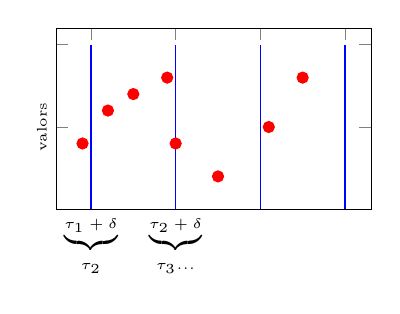
\begin{tikzpicture}
    \begin{axis}[
        width=4cm,
        scale only axis, height=2.3cm,
        ymin = 0,
        yticklabels= {,,\tiny valors},
        y tick label style = {rotate=90,anchor=south},
        x tick label style = {font=\tiny},        
        xticklabels={$\underbrace{\tau_{}}_{\tau_0}$,$\underbrace{\tau_0+\delta}_{\tau_1}$,$\underbrace{\tau_1+\delta}_{\tau_2}$,$\underbrace{\tau_2+\delta}_{\tau_3 \ldots}$},
        ]
 
    \addplot[ycomb,blue] coordinates {
        (20,10)
        (30,10)
        (40,10)
        (50,10)
    }; 

    \addplot[red,only marks, mark = *] coordinates {
        (19,4)
        (22,6)
        (25,7)
        (29,8)
        (30,4)
        (35,2)
        (41,5)
        (45,8)
    };

    \end{axis}
  \end{tikzpicture}





De manera simplificada, hem definit que cada consolidació només
s'aplica a l'interval de consolidació actual; així la consolidació
total del buffer és l'aplicació successiva de l'operació de
consolidació.

Aquesta consolidació successiva requereix que les mesures s'insereixen
al buffer ordenades en el temps, sinó un cop duta a terme la
consolidació les mesures inserides desordenades poden no ser tingudes
en compte. Si es duu a terme aquesta inserció ordenada, aleshores un
buffer té l'estat de consolidable quan el temps d'una mesura de la
sèrie temporal és més gran que el següent instant de temps de
consolidació del buffer.
\begin{definition}[Buffer consolidable]\label{def:model:buffer_consolidable}
  Sigui $B=(S,\tau,\delta,f)$ un buffer, definim que
  \glsdispdef{consolidableB}{$B$ és
    consolidable} si i només si $T(m) \geq \tau+\delta$ a on
  $m=\sup(S)$ és la mesura suprema de la sèrie temporal del buffer.
\end{definition}



\subsubsection{Disc}

Els discs reben les mesures consolidades per a emmagatzemar-les de
forma acotada. Així, tenen un operador associat que afegeix noves
mesures al disc mantenint sota control el seu cardinal.


L'operació d'afegir una mesura al disc consisteix en afegir-la a la
sèrie temporal i a eliminar la mesura mínima d'aquesta si se supera el
cardinal permès.
\begin{definition}[Afegeix mesura al disc]
  Sigui $D=(S,k)$ un disc i $m=(t,v)$ una mesura, la inserció de la
  mesura al disc $\glssymboldef{addD}(D,m)$ és un disc $D'=(S',k)$
  amb la mesura afegida a la sèrie temporal del disc mantenint el
  cardinal màxim: $\glssymbol{addD}(D,m) = (S',k)$ a on $S'=
  \begin{cases}
      S\cup\{m\} &\text{si }  |S|<k\\
      (S-\{\min(S)\}) \cup \{m\} &\text{altrament}
    \end{cases}$.
\end{definition}




\subsubsection{Subsèrie resolució}

Les subsèries resolució són l'aparellament d'un buffer amb un disc.
Així tenen dos operadors associats, els quals treballen amb els
operadors del buffer i del disc : un per afegir una mesura al buffer i
un altre per consolidar el buffer i afegir la mesura resultant al disc


L'operació d'afegir una mesura a la subsèrie resolució consisteix en
afegir-la al buffer.
\begin{definition}[Afegeix mesura a la subsèrie resolució]
  Sigui $R=(B,D)$ una subsèrie resolució i $m=(t,v)$ una mesura, la
  inserció de la mesura a la subsèrie resolució
  $\glssymboldef{addR}(R,m)$ és una subsèrie resolució $R'=(B',D)$
  amb la mesura afegida al buffer: $\glssymbol{addR}(R,m) = (B',D)$ a
  on $B'=\glssymbol{addB}=(B,m)$.
\end{definition}


L'operació de consolidar una subsèrie resolució consisteix en calcular
una mesura de consolidació del buffer, en l'interval de consolidació
actual, i desar-la al disc. 
\begin{definition}[Consolida la subsèrie resolució]
  Sigui $R=(B,D)$ una subsèrie resolució, la consolidació de la
  subsèrie resolució $\glssymboldef{consolidaR}(R)$ és una subsèrie
  resolució $R'=(B',D')$ a on $(B',m') = \glssymbol{consolidaB}(B)$ i
  $D'=\glssymbol{addD}(D,m')$.
\end{definition}

Una subsèrie resolució és consolidable quan ho és el seu buffer.
\begin{definition}[Subsèrie resolució consolidable]
  Sigui $R=(B,D)$ una subsèrie resolució, definim que
  \glsdispdef{consolidableR}{$R$ és
    consolidable} si i només si \glsdisp{consolidableB}{$B$ és
    consolidable}
\end{definition}



\subsubsection{Sèrie temporal multiresolució}

Les sèries temporals multiresolució són un conjunt de subsèries
resolució. Així tenen dos operadors per a treballar globalment amb
totes les subèries que contingui: un per a afegir una mesura a cada
subsèrie i un altre per a consolidar cadascuna de les subsèries.


L'operació d'afegir una mesura a la sèrie temporal multiresolució
consisteix en afegir-la a cadascuna de les subsèries resolució.
\begin{definition}[Afegeix mesura a la sèrie temporal multiresolució]
  Sigui $M=\{R_0,\dotsc,R_d\}$ una sèrie temporal multiresolució i
  $m=(t,v)$ una mesura, la inserció de la mesura a la sèrie temporal
  multiresolució $\glssymboldef{addM}(M,m)$ és una sèrie temporal
  multiresolució $M'=\{R_0',\dotsc,R_d'\}$ amb la mesura afegida a
  cada subsèrie resolució: $\glssymbol{addM}(M,m) = \{ \forall R_i\in
  M: \glssymbol{addR}(R_i,m) \}$.
\end{definition}


L'operació de consolidar una sèrie temporal multiresolució consisteix
en consolidar cadascuna de les subsèries resolució que siguin
consolidables.
\begin{definition}[Consolida la sèrie temporal multiresolució]
  Sigui $M=\{R_0,\dotsc,R_d\}$ una sèrie temporal multiresolució, la
  consolidació de la sèrie temporal multiresolució
  $\glssymboldef{consolidaM}(M)$ és una sèrie temporal multiresolució
  $M'=\{R_0',\dotsc,R_d'\}$ que consolida les subsèries resolució
  consolidables:
  \[
  \glssymbol{consolidaM}(M) = \big\{ \forall R_i\in M:
  \begin{cases}
    \glssymbol{consolidaR}(R_i) & \text{si }
    \glsdisp{consolidableR}{R_i \text{ és
        consolidable}}\\
    R_i & \text{altrament}
  \end{cases}\big\}
  \].
\end{definition}



Una sèrie temporal multiresolució és un conjunt de subsèries
resolució. Per a tractar amb tots i cadascun dels elements del conjunt
és útil tenir l'operació de mapatge, de manera similar a com s'ha
definit per les sèries temporals però que es pugui obtenir qualsevol
conjunt de valors.
 \begin{definition}[Mapa d'una sèrie temporal multiresolució] %angl. span
   Sigui $M=\{R_0,\dotsc,R_d\}$ una sèrie temporal multiresolució i
   \glssymbol{not:F} una funció sobre una subsèrie resolució que
   retorna un valor $v'$ a on $\glssymbol{not:F}:R\mapsto v'$, el mapa
   de \glssymbol{not:F} a $M$ és un conjunt de valors resultant
   d'aplicar la funció a cada subsèrie resolució:
   $\glssymboldef{not:sgstm:map}(M,\glssymbol{not:F}) = \{
   \glssymbol{not:F}(R_0), \dotsc, \glssymbol{not:F}(R_d) \}$.
\end{definition}
Atès que una sèrie temporal multiresolució és un conjunt de subsèries
resolució, un dels resultats possible del mapa és una nova sèrie
temporal multiresolució si la funció és de la forma
$\glssymbol{not:F}:R\mapsto R'$.


% Aplicació de fold a una BDM
% \begin{gather*}
%   \text{fold}: M \times M_i \times f \longrightarrow M' :\\
%   = f(\dots(f(f(f(M_i,R_0),R_1),R_2)\dots),R_k), \\
%    \text{a on } f: M_a \times R_b \mapsto M'
% \end{gather*}





\subsection{Manipulació de l'esquema}
\label{sec:model:sgstm-manipulacio-esquema}
\todo{alerta! aquesta secció s'ha fet pensant en els instants de consolidació periòdics. Què passa quan no ho són? }
per exemple event trigerred (només emmatgatzemem informació quan creiem que és interessant). Aleshores potser són casos molt especials i no es pot dibuixar l'esquema? Potser posar tot això com a comentari a la secció d'Altres Estructures: En el model de \gls{SGSTM} s'ha considerat que la consolidació es feia periòdicament però es podria fer quan es cregués oportú, aleshores no es pot preveure quin esquema de multiresolució hi haurà; són casos que requereixen un estudi més profund. Etc.

\todo{atenció que no s'ha parlat enlloc del rellotge en els SGBDM? s'hauria de dir que en principi no es diu res sobre el rellotge i que si segueix l'esquema de consolidació proposat les mateixes mesures van entrant ordenades i van marcant el pas del temps}



El model de \gls{SGSTM} associa a cada sèrie temporal un esquema de
multiresolució. En aquest apartat definim els operadors que permeten
consultar i manipular aquest esquema de multiresolució de forma
coherent amb el model de \gls{SGSTM}.

L'\glsdispsec{not:esquemaM}{esquema de multiresolució} de
cada sèrie temporal multiresolució consisteix en quatre paràmetres
variables: el darrer instant de consolidació ($\tau$), el pas de
consolidació ($\delta$), el cardinal màxim ($k$) i la funció
d'agregació d'atributs ($f$).

Així doncs, quan es manipula una base de dades multiresolució cal
conservar o tractar adequadament aquest esquema de multiresolució.  A
continuació es descriuen operadors per a poder estudiar aquest
esquema, operadors per a canviar-lo i operadors per a unir o ajuntar
dos esquemes.


A cada sèrie temporal multiresolució li correspon un esquema de
multiresolució.  Una sèrie temporal multiresolució és un conjunt de
subsèries resolució i per tant l'esquema de multiresolució és també un
conjunt de l'esquema de cada subsèrie.  A continuació definim els
operadors de manipulació per a les subsèries resolució, els quals es
poden estendre fàcilment a una sèrie temporal multiresolució
mitjançant l'operació de mapatge.




\subsubsection{Propietats de l'esquema}

La configuració dels quatre paràmetres variables de l'esquema de
multiresolució confereix una sèrie de propietats als objectes d'una
base de dades multiresolució. A continuació definim algunes propietats
que es poden estudiar a partir d'un esquema de multiresolució.


Donat un esquema de multiresolució podem dibuixar la situació relativa
en el temps que prendran les mesures. A aquest dibuix de l'esquema de
multiresolució l'anomenem cronograma. Per exemple, sigui la sèrie
temporal multiresolució $M^d=\{R_0,R_1\}$ de
l'\autoref{ex:model:bdm-desfasaments} dibuixem el seu cronograma a la
\autoref{fig:model:cronograma} per a l'instant de temps $30$, just
abans de la seva consolidació. Les subsèries resolució de $M^d$ tenen
els paràmetres $\delta_0=5$, $\delta_1=10$, $k_1=4$, $k_2=3$,
$f_1=\text{mitjana}$ i $f_2=\text{mitjanad5}$ a on la funció
$\text{mitjanad5}$ té un desfasament de $5$ unitats de temps. Tot
seguit definim els conceptes que apareixen al cronograma.

\begin{figure}[tp]
  \centering
  %\usetikzlibrary{positioning}
\begin{tikzpicture}

  %referencia
  \def\ut{1.2}
  \node (-10) {};

  \foreach \x in {-9,...,0}
  {
    \pgfmathparse{int(\x-1)}
    \let\antx=\pgfmathresult 
    \pgfmathparse{int(5*\x+30)}
    \let\nomx=\pgfmathresult
    
    \node[align=center] (\x) [right=\ut cm of \antx.center,anchor=center] {
    %  \x
    \nomx  %noms de les x
    };
    \node [above=0mm of \x] {\tiny$\vert$};
  }



  %eixos
  \node (et0) [above=0mm of 0] {};
  \node (eti) [left=11cm of et0] {};
  \node (etf) [right=0.5cm of et0] {};
  \draw[->] (eti) to (etf);
  \node [below=2mm of -10,anchor=west] {temps (u.t.)};

  \node (ara) [above=4cm of et0] {};
  \node (ara2) [below=5mm of et0] {};
  \draw[-] (ara) to (ara2);
  \node (ara3) [below=-2mm of ara2] {};

  


 %R1 d2 k4 tau0 f-1
  \node (R1) [above=1cm of 0] {};
  \node[ellipse,draw,minimum width=3*\ut cm] (R1b) [left=0mm of R1.center, anchor=east] {$S_{B2}$};
  \node[rectangle,draw,minimum width=2*\ut cm] (R1d1) [left=0mm of R1b.west, anchor=east] {$S_{D2}^1$};
  \node[rectangle,draw,minimum width=2*\ut cm,align=center] (R1d2) [left=0mm of R1d1.west, anchor=east] {$S_{D2}^2$};
  \node[rectangle,draw,minimum width=2*\ut cm,align=center] (R1d3) [left=0mm of R1d2.west, anchor=east] {$S_{D2}^3$};



  %R0 d1 k4 tau0
  \node (R0) [above=2.5cm of R1.center] {};
  \node[ellipse,draw,minimum width=\ut cm,align=center] (R0b) [left=0mm of R0.center, anchor=east] {$S_{B1}$};
  \node[rectangle,draw,minimum width=\ut cm,align=center] (R0d1) [left=0mm of R0b.west, anchor=east] {$S_{D1}^1$};
  \node[rectangle,draw,minimum width=\ut cm,align=center] (R0d2) [left=0mm of R0d1.west, anchor=east] {$S_{D1}^2$};
  \node[rectangle,draw,minimum width=\ut cm,align=center] (R0d3) [left=0mm of R0d2.west, anchor=east] {$S_{D1}^3$};
  \node[rectangle,draw,minimum width=\ut cm,align=center] (R0d4) [left=0mm of R0d3.west, anchor=east] {$S_{D1}^4$};


  %definicions
  \node (R0la) [above=5mm of R0d4.west] {};
  \node (R0lb) [above=5mm of R0d1.east] {};
  \draw[<->] (R0la.center) -- (R0lb.center) node [above,sloped,midway] {$lapseR(R_1)$};

  \node (R1la) [above=5mm of R1d3.west] {};
  \node (R1lb) [above=5mm of R1d1.east] {};
  \draw[<->] (R1la) -- (R1lb) node [above,sloped,midway] {$lapseR(R_2)$};


  \node (R0ba) [above=5mm of R0b.west] {};
  \node (R0bb) [above=5mm of R0b.east] {};
  \draw[<->] (R0ba) -- (R0bb) node [above,sloped,midway] {$periodeB(R_1)$};

  \node (R1ba) [above=12mm of R1b.west] {};
  \node (R1bb) [above=12mm of R1b.east] {};
  \draw[<->] (R1ba) -- (R1bb) node [above,sloped,midway] {$periodeB(R_2)$};

  \node (R1da) [above=5mm of R1b.west] {};
  \node (R1db) [above=5mm of -2] {};
  \draw[<->] (R1da.center) -- (R1da-|R1db) node [above,sloped,midway] {$desfasamentR(R_2)$};

  \node [below=0mm of -1] {$\tau_1$};
  \node [below=0mm of -2] {$\tau_2$};
  \node (tau0d) [below=0mm of 0] {$\tau_1+\delta_1$};
  \node [below=0mm of tau0d] {$\tau_2+\delta_2$};

\end{tikzpicture}
  \caption{Cronograma d'un esquema multiresolució just abans de la consolidació, a on $\glssymbol{not:sgstm:periodeB}(R_i)=\glssymbol{not:sgstm:lapseB}(R_i)$}
  \label{fig:model:cronograma}
\end{figure}


Els paràmetres $k$, $\delta$ i $f$ d'una subsèrie resolució són fixats
per l'esquema, mentre que el paràmetre $\tau$ és fixat a un valor
inicial i va sent canviat per l'operació de consolidar. Així doncs,
les propietats que impliquin a $\tau$ dependran de l'instant temporal
en que es faci la consulta i les que no l'impliquin seran fixes per a
cada esquema.

Una propietat que observem en el cronograma és el lapse temporal d'una
subsèrie resolució; és a dir una mesura de la mida temporal que ocupa
la subsèrie temporal emmagatzemada en el seu disc.
\begin{definition}[Lapse de la subsèrie resolució] %angl. span
  Sigui $R=(S_B,S_D,\tau,\delta,k,f)$ una subsèrie resolució, el seu
  lapse $\glssymboldef{not:sgstm:lapseR}(R)$ és una durada de temps $t^d$
  que mesura la mida de l'interval que ocupa el disc:
  $\glssymbol{not:sgstm:lapseR}(R) = k\delta$.
\end{definition}


Si definim l'interval del lapse com a $[\tau - k\delta, \tau]$
i l'interval temporal real de la sèrie temporal del disc com a
$[\min(S_D),\max(S_D)]$, aleshores normalment es complirà que
$\max(S_D)=\tau$ i $\min(S_D)=\tau - (k-1)\delta$. No obstant, això
pot no complir-se si la sèrie temporal no és regular, si $\tau$ i
$\max(S_D)$ no coincideixen, etc. 

Quan $\tau$ i $\max(S_D)$ no coincideixen és degut a un desfasament
provocat per la funció d'agregació i ho anomenem desfasament de la
subsèrie resolució.
\begin{definition}[Desfasament de la subsèrie resolució] %angl. offset
  \label{def:sgstm:desdsamentR}
  Sigui $R=(S_B,S_D,\tau,\delta,k,f)$ una subsèrie resolució, el seu
  desfasament $\glssymboldef{not:sgstm:desfasamentR}(R)$ és una durada de
  temps $t^d$ que mesura la distància entre $\tau$ i $\max(S_D)$
  deguda a la funció d'agregació $f$. Així havent definit la
  consolidació sobre $m'=f(S,[\tau,\tau+\delta]$
  (v.~\autoref{def:model:consolidacio-buffer}), la funció d'agregació
  amb desfasament retornarà una mesura $m'=(\tau - r,v)$ a on
  $\glssymbol{not:sgstm:desfasamentR}(R) = r$.
\end{definition}


Un altre desfasament que es produeix, aquest però variable, és la
variació que hi ha entre el darrer instant de consolidació i l'instant
de temps actual. Aquest interval de temps és durant el qual el buffer
emmagatzema les noves mesures que arriben i l'anomenen període de
buffer.
\begin{definition}[Període de buffer de la subsèrie resolució]
  Sigui $R=(S_B,S_D,\tau,\delta,k,f)$ una subsèrie resolució,
  $\glssymbol{not:sgstm:desfasamentR}(R)$ el seu desfasament i $t^n$
  l'instant de temps actual, el període de buffer de la subsèrie
  resolució $\glssymboldef{not:sgstm:periodeB}(R)$ és una durada de temps
  $t^d$ que mesura la distància entre $\tau$ i $t^n$ tenint en compte
  el desfasament: $\glssymbol{not:sgstm:periodeB}(R) = t^n - (\tau -
  \glssymbol{not:sgstm:desfasamentR}(R))$.
\end{definition}

Si la consolidació de la subsèrie resolució es realitza immediatament
cada cop que estigui en estat de consolidable, aleshores el període de
buffer té una variació limitada atès que fent la consolidació
immediata $t^n - \tau \leq \delta$. El mínim que pot prendre el
període de buffer de la subsèrie resolució és $\glssymbol{not:sgstm:desfasamentR}(R)$
i al màxim l'anomenem lapse de buffer de la subsèrie resolució.
\begin{definition}[Lapse de buffer de la subsèrie resolució]
  Sigui $R=(S_B,S_D,\tau,\delta,k,f)$ una subsèrie resolució i
  $\glssymbol{not:sgstm:desfasamentR}(R))$ el seu desfasament, el
  lapse de buffer de la subsèrie resolució
  $\glssymboldef{not:sgstm:lapseB}(R)$ és una durada de temps $t^d$ que
  mesura el període de buffer màxim que pot prendre:
  $\glssymbol{not:sgstm:lapseB}(R) = \delta +
  \glssymbol{not:sgstm:desfasamentR}(R)$.  Sempre es compleix que
  $\glssymbol{not:sgstm:periodeB}(R) \leq
  \glssymbol{not:sgstm:lapseB}(R)$ atès que fent la consolidació
  immediata $t^n - \tau \leq \delta$.
\end{definition}


Una altra propietat de l'esquema de multiresolució és la
regularització de les sèries temporals emmagatzemades en el disc. El
període d'aquesta sèrie temporal del disc normalment es correspondrà
amb $\delta$. No obstant, notem que en determinats instants això pot
no complir-se com per exemple durant un canvi en l'esquema del pas de
consolidació. Donades dues subsèries resolució i tenint en compte el
període de la sèrie temporal, podem establir quina d'elles conté més
resolució.
\begin{definition}[Subsèrie resolució amb més resolució]
  Siguin $R_1=(S_{B1},S_{D1},\tau_1,\delta_1,k_1,f_1)$ i
  $R_2=(S_{B2},S_{D2},\tau_2,\delta_2,k_2,f_2)$ dues subsèries
  resolució, la subsèrie amb més resolució
  $\glssymboldef{not:sgstm:maxR}(R_1,R_2)$ és la que té el pas de
  consolidació més petit: $\glssymbol{not:sgstm:maxR}(R_1,R_2) = R_i$
  a on $\delta_i = \min(\delta_1,\delta_2)$.
\end{definition}



Resumint, podem dir que una subsèrie resolució té, per una
banda, informació consolidada per un lapse temporal de
$\glssymbol{not:sgstm:lapseR}(R)$ el qual es posiciona absolutament des de $\tau +
\glssymbol{not:sgstm:desfasamentR}(R)$ enrere. Per altra banda, la subsèrie resolució
té informació no consolidada al davant de la consolidada per un
interval de mida $\glssymbol{not:sgstm:periodeB}(R)$ i de com a màxim
$\glssymbol{not:sgstm:lapseB}(R)$. 

A la \autoref{fig:model:cronograma} s'ha pogut observar totes les
propietats definides pel cronograma multiresolució. Aquest cronograma
mostra una fotografia a l'instant de temps determinat, el $30$, que es
correspon amb un moment abans que es consolidin les dues subsèries
resolució. Aquest és un moment a on es compleix la
propietat$\glssymbol{not:sgstm:periodeB}(R_i)=\glssymbol{not:sgstm:lapseB}(R_i)$; és a dir a on el
període de buffer té la mida màxima.

\begin{figure}[tp]
  \centering
  %\usetikzlibrary{positioning}
\begin{tikzpicture}

  %referencia
  \def\ut{1.2}
  \node (-8) {};

  \foreach \x in {-7,...,2}
  {
    \pgfmathparse{int(\x-1)}
    \let\antx=\pgfmathresult
    \pgfmathparse{int(5*\x+30)}
    \let\nomx=\pgfmathresult

    \node[align=center] (\x) [right=\ut cm of \antx.center,anchor=center] {
    %  \x
    \nomx  %noms de les x      
    };
    \node [above=0mm of \x] {\tiny$\vert$};
  }


  %eixos
  \node (et0) [above=0mm of 0] {};
  \node (eti) [left=8.5cm of et0] {};
  \node (etf) [right=3cm of et0] {};
  \draw[->] (eti) to (etf);
  \node [below=2mm of -8,anchor=west] {temps (u.t.)};

  \node (ara) [above=4cm of et0] {};
  \node (ara2) [below=5mm of et0] {};
  \draw[-] (ara) to (ara2);
  \node (ara3) [below=-2mm of ara2] {};

  


 %R1 d2 k4 tau0 f-1
  \node (R1) [above=1cm of 0] {};
  \node[ellipse,draw,minimum width=\ut cm] (R1b) [left=0mm of R1.center, anchor=east] {$S_{B1}$};
  \node[rectangle,draw,minimum width=2*\ut cm] (R1d1) [left=0mm of R1b.west, anchor=east] {$S_{D1}^1$};
  \node[rectangle,draw,minimum width=2*\ut cm,align=center] (R1d2) [left=0mm of R1d1.west, anchor=east] {$S_{D1}^2$};
  \node[rectangle,draw,minimum width=2*\ut cm,align=center] (R1d3) [left=0mm of R1d2.west, anchor=east] {$S_{D1}^3$};



  %R0 d1 k4 tau0
  \node (R0) [above=2cm of R1.center] {};
%  \node[ellipse,draw,minimum width=\ut cm,align=center] (R0b) [left=0mm of R0.center, anchor=east] {$S_{B1}$};
  \node[rectangle,draw,minimum width=\ut cm,align=center] (R0d1) [left=0mm of R0.center, anchor=east] {$S_{D0}^1$};
  \node[rectangle,draw,minimum width=\ut cm,align=center] (R0d2) [left=0mm of R0d1.west, anchor=east] {$S_{D0}^2$};
  \node[rectangle,draw,minimum width=\ut cm,align=center] (R0d3) [left=0mm of R0d2.west, anchor=east] {$S_{D0}^3$};
  \node[rectangle,draw,minimum width=\ut cm,align=center] (R0d4) [left=0mm of R0d3.west, anchor=east] {$S_{D0}^4$};


  %definicions
  \node (R0la) [above=5mm of R0d4.west] {};
  \node (R0lb) [above=5mm of R0d1.east] {};
  \draw[<->] (R0la.center) -- (R0lb.center) node [above,sloped,midway] {$lapseR(R_0)$};

  \node (R1la) [above=5mm of R1d3.west] {};
  \node (R1lb) [above=5mm of R1d1.east] {};
  \draw[<->] (R1la) -- (R1lb) node [above,sloped,midway] {$lapseR(R_1)$};


%  \node (R0ba) [above=5mm of R0b.west] {};
%  \node (R0bb) [above=5mm of R0b.east] {};
%  \draw[<->] (R0ba) -- (R0bb) node [above,sloped,midway] {$periodeB(R_0)$};

  \node (R1ba) [above=5mm of R1b.west] {};
  \node (R1bb) [above=5mm of R1b.east] {};
  \draw[<->] (R1ba) -- (R1bb) node [above,sloped,midway] {$periodeB(R_1)$};

  % \node (R1da) [above=5mm of R1b.west] {};
  % \node (R1db) [above=5mm of -2] {};
  % \draw[<->] (R1da.center) -- (R1da-|R1db) node [above,sloped,midway] {$desfasamentB(R_1)$};


  \node (tau0d) [below=0mm of 0] {$\tau_0$};
  \node [below=0mm of tau0d] {$\tau_1$};
  \node [below=0mm of 1] {$\tau_0+\delta_0$};
  \node [below=0mm of 2] {$\tau_1+\delta_1$};

\end{tikzpicture}
  \caption{Cronograma d'un esquema multiresolució just després de la consolidació, a on $\glssymbol{not:sgstm:periodeB}(R_i)=\glssymbol{not:sgstm:desfasamentR}(R_i)$}
  \label{fig:model:cronograma-consolidat}
\end{figure}

El cronograma canvia amb el pas del temps; és a dir canvia la mida
dels buffers i la posició temporal dels discs. Es pot veure a la
\autoref{fig:model:cronograma-consolidat} a on s'ha dibuixat l'exemple anterior
però en instant de temps $30$ just després de la consolidació de les
dues subsèries resolució. Aquest és un moment a on es compleix la
propietat $\glssymbol{not:sgstm:periodeB}(R_i)=\glssymbol{not:sgstm:desfasamentR}(R_i)$; és a dir a
on el període de buffer té la mida mínima.  


\begin{figure}[tp]
  \centering
  \begin{tikzpicture}

  %R0
  \node[circle,draw,minimum width=2 cm] (R0d) {$\delta_{0}$};
  \draw [->] (R0d.center)++(.4:.4cm) arc(0:180:.4cm);

  \node[circle,draw] [left=0mm of R0d.north,anchor=center] {};
  \node[circle,draw] [left=0mm of R0d.east,anchor=center] {};
  \node[circle,draw] [left=0mm of R0d.south,anchor=center] {};
  \node[circle,draw] [left=0mm of R0d.west,anchor=center] {};

  %R1
  \node[circle,draw,minimum width=2 cm] (R1d) [right=of R0d] {$\delta_{1}$};
  \draw [->] (R1d.center)++(.4:.4cm) arc(0:180:.4cm);

  \node[circle,draw] [left=0mm of R1d.north,anchor=center] {};
  \node[circle,draw] [left=0mm of R1d.south west,anchor=center] {};
  \node[circle,draw] [left=0mm of R1d.south east,anchor=center] {};

\end{tikzpicture}
\begin{tikzpicture}

  %referencia
  \def\ut{1.2}
  \node (-8) {};

  \foreach \x in {-7,...,0}
  {
    \pgfmathparse{int(\x-1)}
    \let\antx=\pgfmathresult
    \pgfmathparse{int(5*\x)}
    \let\nomx=\pgfmathresult

    \node[align=center] (\x) [right=\ut cm of \antx.center,anchor=center] {
    %  \x
    \nomx  %noms de les x      
    };
    \node [above=0mm of \x] {\tiny$\vert$};
  }


  %eixos
  \node (et0) [above=0mm of 0] {};
  \node (eti) [left=8.5cm of et0] {};
  \node (etf) [right=0.5cm of et0] {};
  \draw[->] (eti) to (etf);
  \node [below=2mm of -8,anchor=west] {temps (u.t.)};

  \node (ara) [above=3cm of et0] {};
  \node (ara2) [below=5mm of et0] {};
  \draw[-] (ara) to (ara2);
  \node (ara3) [below=-2mm of ara2] {};

  


 %R1 d2 k4 tau0 f-1
  \node (R1) [above=1cm of 0] {};
  \node[rectangle,draw,minimum width=6*\ut cm] (R1d) [left=\ut cm of R1.center, anchor=east] {$\text{lapseR}(R_2)$};




  %R0 d1 k4 tau0
  \node (R0) [above= of R1.center] {};
  \node[rectangle,draw,minimum width=4*\ut cm] (R0d) [left=0 cm of R0.center, anchor=east] {$\text{lapseR}(R_1)$};
\end{tikzpicture}

  \caption{Cronograma periòdic d'un esquema multiresolució}
  \label{fig:model:cronograma-simplificat}
\end{figure}

Així doncs, el cronograma evoluciona amb el temps i a cada instant
determinat presenta una forma. No obstant, les formes es repeteixen
periòdicament en el temps; el període de repetició és de $\delta$ per
a cada subsèrie resolució. Per a simplificar dibuixarem un cronograma
que només mostri aquesta informació periòdica; així establirem
l'instant 0 com aquell on totes les subsèries resolució es consoliden
al mateix temps i dibuixarem els lapses enrere en el temps. A la
\autoref{fig:model:cronograma-simplificat} es pot veure el cronograma
periòdic per als exemples anteriors a on l'eix del temps ens indica
les durades i les posicions relatives dels discs de les subsèries
resolució. La informació referent al pas de consolidació i la
resolució dels discs es dibuixa a la part superior amb formes
circulars, de manera que s'observa clarament quina subsèrie té més
resolució.



\subsubsection{Canvis de l'esquema}

Canviar l'esquema multiresolució d'una sèrie temporal significa crear
un esquema nou de multiresolució i emmagatzemar-hi les dades de
l'esquema vell de forma que es conservi la coherència que tenien
aquestes dades. Així doncs, a continuació definim algunes operacions
de canvi d'esquema que es poden aplicar als objectes d'una base de
dades multiresolució de forma coherent amb les dades emmagatzemades.


L'operació que canvia la mida del disc d'una subsèrie resolució ha de
controlar que si la mida disminueix s'han d'eliminar dades.
\begin{definition}[Canvi de mida d'una subsèrie resolució]
  Sigui $R=(B,D)$ una subsèrie resolució, a on $D=(S_D,k)$ és el disc
  de la subsèrie, i $k'$ un nou cardinal màxim, el canvi de mida de la
  subsèrie resolució $\glssymboldef{not:sgstm:canviaK}(R,k')$ és una
  nova subsèrie resolució $R'=(B,D')$ amb les dades antigues afegides
  de nou al disc: $\glssymbol{not:sgstm:canviaK}(R,k')= (B,D')$ a on
  s'aplica l'operació $\forall m_i \in S_D: \glssymbol{addD}(D',m_i)$
  amb $D'=(\{\},k')$ com a disc inicial.
\end{definition}


L'operació que canvia el pas de consolidació d'una subsèrie resolució
no cal que tingui en compte les dades ja que la sèrie temporal
emmagatzemada s'anirà canviant quan es consolidin noves mesures.
\begin{definition}[Canvi de pas de consolidació d'una subsèrie resolució]
  Sigui $R = (S_B,S_D,\delta,\tau,k,f)$ una subsèrie resolució i
  $\delta'$ un nou pas de consolidació, el canvi del pas de
  consolidació de la subsèrie resolució
  $\glssymboldef{not:sgstm:canviad}(R,\delta')$ és la nova subsèrie resolució
  $\glssymbol{not:sgstm:canviad}(R,\delta')=(S_B,S_D,\delta',\tau,k,f)$.
\end{definition}

Hi ha altres canvis de l'esquema que tampoc no requereixen tenir en
compte les dades, com per exemple canviar la funció d'agregació
d'atribut. Atès que són molt semblants al canvi de pas de
consolidació, no definim operadors específics per a aquestes
operacions.


L'operació que canvia la resolució d'una subsèrie resolució modifica
alhora la mida i el pas de consolidació tenint en compte les dades; és
a dir, canvia el període de la sèrie temporal emmagatzemada seguint el
criteri de representació.
\begin{definition}[Canvi de resolució d'una subsèrie resolució]
  Sigui $R = (S_B,S_D,\delta,\tau,k,f)$ una subsèrie resolució, $r$
  una funció de representació per a la sèrie temporal, $k'$ un nou
  cardinal màxim i $\delta'$ un nou pas de consolidació, el canvi de
  resolució de la subsèrie resolució
  $\glssymboldef{not:sgstm:canviaR}(R,k',\delta')$ és una nova subsèrie
  resolució $R' = (S_B,S_D',\delta',\tau,k',f)$ amb una selecció
  temporal segons el criteri de representació en el nou conjunt
  regular de temps:
  $\glssymbol{not:sgstm:canviaR}(R,k',\delta')=(S_B,S_D',\delta',\tau,k',f)$
  a on $S_D' = S_D[T]^r$ i $T=\{ \tau-n\delta' | n\in\mathbb{N},n<k'
  \}$.
\end{definition}


Per a treballar amb sèries temporals multivaluades cal que les sèries
temporals emmagatzemades als buffers i al discs tinguin la mateixa
forma. Així afegir un nou multivalor significa afegir un nou atribut a
les sèries temporals del buffer i dels disc de cada subsèrie
resolució. A continuació definim com afegir un multivalor a una
subsèrie resolució considerant sèries temporals en la forma canònica;
a la pràctica, per comoditat, habitualment cada atribut de multivalor
tindrà un nom.
\begin{definition}[Afegeix multivalor a una subsèrie resolució]
  Sigui $R = (S_B,S_D,\delta,\tau,k,f)$ una subsèrie resolució,
  l'addició d'un nou multivalor és una subsèrie resolució
  $\glssymboldef{not:sgstm:addMV}(R) = (S_B',S_D',\delta,\tau,k,f)$ amb les
    sèries temporals ampliades amb un nou atribut inicialment de valor
    indefinit $S'_{B} = \map(S_B,(t,v)\mapsto(t,(v,\infty)))$ i
    $S'_{D} = \map(S_D,(t,v)\mapsto(t,(v,\infty)))$.
\end{definition}





\subsubsection{Unió i junció de dos esquemes}

Dos casos particulars de canvi d'esquema multiresolució són el d'unió
i el de junció de dos esquemes. En aquests canvis cal crear un nou
esquema tot conservant la coherència de dades emmagatzemades en dos
esquemes diferents.

Un exemple d'aplicació de la unió de dos esquemes és el següent. Es
mesuren els valors d'una sèrie temporal i durant un temps
s'emmagatzemen com a sèrie temporal multiresolució en una base de
dades però durant un altre temps s'emmagatzemen en una altra base de
dades. En acabar es volen unir els valors emmagatzemats a les dues
bases de dades.

Un exemple d'aplicació de la junció de dos esquemes és el següent.  Es
mesuren els valors de dues sèries temporals diferents i s'emmagatzemen
com a dues sèries temporals multiresolució diferents. En acabar es
volen ajuntar els dos valors en una mateixa sèrie temporal
multivaluada.



L'operació d'unió de dues subsèries resolució és una unió de les
sèries temporals de cada un.
\begin{definition}[Unió de dues subsèries resolució]
  Sigui $R_1=(S_{B1},S_{D1},\delta_1,\tau_1,k_1,f_1)$ i
  $R_2=(S_{B2},S_{D2},\delta_2,\tau_2,k_2,f_2)$ dues subsèries
  resolució, la unió de les dues subsèries resolució
  $\glssymboldef{not:sgstm:unioR}(R_1,R_2)$ és una subsèrie resolució $R' =
  (S'_B,S'_D,\delta',\tau',k',f')$ que conté la unió de les sèries
  temporals dels seus buffers i discs: $\glssymbol{not:sgstm:unioR}(R_1,R_2)=
  (S'_B,S'_D,\delta_1,\max(\tau_1,\tau_2),k_1+k_2,f_1)$ a on $S'_B =
  S_{B1} \cup S_{B2}$ i $S'_D = S_{D1} \cup S_{D2}$.
\end{definition}
La unió de dues subsèries resolució no és commutativa degut a que les
unions de les sèries temporals no ho són. Tampoc ho és degut a que si
s'uneixen dues subsèries resolució amb diferent $\delta$ i $f$ llavors
es determina que la primera marca quins són els $\delta'$ i $f'$
resultants.  És a dir que en cas que es vulguin unir subsèries
resolució que continguin mesures en el mateix temps o informació
diferent; es prioritza la primera.


L'operació d'unió de dues sèries temporals multiresolució és la unió
de conjunts per a les subsèries resolució quan no intersequen en les
claus $(\delta,f)$. En cas que intersequin cal unir les dues subsèries
resolució.
\begin{definition}[Unió de dues sèries temporals  multiresolució]
  Sigui $M_1=\{R_0^1,\dotsc,R_{d1}^1\}$ i
  $M_2=\{R_0^2,\dotsc,R_{d2}^2\}$ dues sèries temporals
  multiresolució, la unió de les dues
  $\glssymboldef{not:sgstm:unioM}(M_1, M_2)$ és una sèrie temporal
  multiresolució $M'=\{R_0',\dotsc,R_d'\}$ que conté les subsèries que
  no intersequen i la unió de les subsèries que intersequen:
  $\glssymbol{not:sgstm:unioM}(M_1, M_2)= M_{a} \cup M'_{1} \cup
  M'_{2}$ a on $M_a = \{\forall R_1\in M_1,R_2\in M_2:
  \glssymbol{not:sgstm:unioR}(R_1,R_2) | (\delta_1,f_1) =
  (\delta_2,f_2) \}$, $M_1' =\{\forall R_1\in M_1: R_1 | \nexists R_2
  \in M_2 : (\delta_1,f_1) = (\delta_2,f_2) \}$ i $M_2' =\{\forall
  R_2\in M_2: R_2 | \nexists R_1 \in M_1 : (\delta_1,f_1) =
  (\delta_2,f_2) \}$.
\end{definition}
La unió de dues sèries temporals multiresolució no és commutativa
degut a que la unió de subsèries resolució no ho és.





L'operació de junció de dues subsèries resolució és la fusió de les
dades de les dues en una sèrie temporal multivalor. En el cas que els
vectors de temps siguin els mateixos es pot utilitzar la junció de
sèries temporals. En el cas que alguns temps no coincideixin cal
utilitzar la junció temporal amb una representació que donarà valors
allà on manquin.
\begin{definition}[Junció de dues subsèries resolució]
  Sigui $R_1=(S_{B1},S_{D1},\delta_1,\tau_1,k_1,f_1)$ i
  $R_2=(S_{B2},S_{D2},\delta_2,\tau_2,k_2,f_2)$ dues subsèries
  resolució i $r$ una funció de representació de sèries temporals, la
  junció de les dues subsèries resolució
  $\glssymboldef{not:sgstm:joinR}^r(R_1,R_2)$ és una subsèrie
  resolució $R' = (S'_B,S'_D,\delta',\tau',k',f')$ que conté la junció
  temporal de les sèries temporals dels seus buffers i discs:
  $\glssymbol{not:sgstm:joinR}^r(R_1,R_2)=
  (S'_B,S'_D,\delta_1,\max(\tau_1,\tau_2),k_1+k_2,f_1)$ a on $S'_B =
  S_{B1} \join^r S_{B2}$ i $S'_D = S_{D1} \join^r S_{D2}$.
\end{definition}
La junció de dues subsèries resolució no és commutativa degut a que si
s'uneixen dues subsèries resolució amb diferent $\delta$ i $f$ llavors
es determina que la primera marca quins són els $\delta'$ i $f'$
resultants.



L'operació de junció de dues sèries temporals multiresolució
és la unió de conjunts per a les subsèries resolució, ampliades amb un
multivalor indefinit, quan no intersequen en les claus $(\delta,f)$. En
cas que intersequin cal ajuntar les dues subsèries resolució.
\begin{definition}[Junció de dues sèries temporals multiresolució]
  Sigui $M_1=\{R_0^1,\dotsc,R_{d1}^1\}$ i
  $M_2=\{R_0^2,\dotsc,R_{d2}^2\}$ dues sèries temporals multiresolució
  i $r$ una funció de representació de sèries temporals, la junció de
  les dues $\glssymboldef{not:sgstm:joinM}^r(M_1, M_2)$ és una sèrie
  temporal multiresolució $M'=\{R_0',\dotsc,R_d'\}$ que conté les
  subsèries que no intersequen ampliades amb un multivalor i la junció
  de les subsèries que intersequen:
  $\glssymbol{not:sgstm:joinM}^r(M_1, M_2)= M_{a} \cup M'_{1} \cup
  M'_{2}$ a on $M_a = \{\forall R_1\in M_1,R_2\in M_2:
  \glssymbol{not:sgstm:joinR}(R_1,R_2) | (\delta_1,f_1) =
  (\delta_2,f_2) \}$, $M_1' = \{\forall R_1\in M_1:
  \glssymbol{not:sgstm:addMV}(R_1)| \nexists R_2 \in M_2 :
  (\delta_1,f_1) = (\delta_2,f_2) \}$ i $M_2' = \{\forall R_2\in M_2:
  \glssymbol{not:sgstm:addMV}(R_2)| \nexists R_1 \in M_1 :
  (\delta_1,f_1) = (\delta_2,f_2) \}$.
\end{definition}





\subsection{Consultes}

En els sistemes de gestió de bases de dades les consultes són les
operacions que permeten treballar amb les dades emmagatzemades. En el
cas dels \gls{SGSTM} les dades són sèries temporals emmagatzemades amb forma
de multiresolució. Així doncs, els operadors de consulta que es
defineixen a continuació permeten extreure les sèries temporals que hi
ha emmagatzemades amb l'objectiu d’aplicar-hi posteriorment els
operadors propis de les sèries temporals, com s'ha definit en el model
dels \gls{SGST}.

Els \glsdispsec{not:sgstm:consulta}{operadors de consulta} en un \gls{SGSTM}
en primer lloc es basen en obtenir sèries temporals de la base de
dades multiresolució per a en segon lloc aplicar-hi les operacions
dels \gls{SGST}.  En aquest apartat definim el operadors que permeten
obtenir les sèries temporals a partir d'una sèrie temporal
multiresolució; l'aplicació posterior d'operadors a les sèries
temporals segueix les mateixes definicions que en el model
d'operacions dels \gls{SGST} (v.~\autoref{sec:model:sgst-operacions}).

Distingim entre dos tipus d'operadors de consulta. Uns permeten
extreure les subsèries temporals de les subsèries resolució i uns altres
permeten abstreure una sèrie temporal resolució com si fos una sola
sèrie temporal amb diferents períodes de mostreig.


\subsubsection{Extracció de subsèries}


Les subsèries resolució estan caracteritzades per la parella de pas de
consolidació i funció d'agregació d'atributs $(\delta,f)$, ja que són
els atributs clau del conjunt. Seleccionant aquests dos paràmetres
d'una sèrie temporal multiresolució s'obté la subsèrie resolució
corresponent, de la qual es pot extreure la sèrie temporal
emmagatzemada al seu buffer o al seu disc. A continuació mostrem con
seleccionar la sèrie temporal del disc, per a la del buffer es pot
procedir de forma similar.

\begin{definition}[Selecció de la sèrie temporal d'un disc]
  Sigui $M=\{R_0,\dotsc,R_{d}\}$ una sèrie temporal multiresolució, a
  on cada $R_i=(S_{Bi},S_{Di},\delta_i,\tau_i,k_i,f_i)$ és una
  subsèrie resolució, $\delta$ un pas de consolidació i $f$ una funció
  d'agregació d'atributs, la selecció de la sèrie temporal d'un disc
  de la sèrie temporal multiresolució és la sèrie temporal
  $\glssymboldef{not:sgstm:seriedisc}(M,\delta,f)= S'$ a on $S'= S_D' |
  (S_B',S_D',\delta',\tau',k',f) \in M$ sent $S_B'$, $\tau'$ i $k'$ qualsevol
  valor.
\end{definition}




\subsubsection{Sèrie temporal total}

%Alerta: en el punt d'unió de les conatenacions queda mal unit perquè el valor de més resolució fa un span més gros del que li toca



La sèrie temporal total és la sèrie temporal que ofereix la màxima
resolució de la sèrie temporal multiresolució; és a dir que concatena
les subsèries resolució tenint en compte el pas de consolidació de
cada una. El resultat és una sèrie temporal amb períodes de mostreig
regulars a trossos.
\begin{definition}[Sèrie temporal total]
  Sigui $M^*=\{R_0,\dotsc,R_{d}\}$ una sèrie temporal multiresolució a
  on no hi ha $\delta$ repetits, la sèrie temporal total de la sèrie
  temporal multiresolució $\glssymboldef{not:sgstm:serietotal}(M^*)$
  és la sèrie temporal que resulta de la concatenació de les sèries
  temporals dels discs per ordre de pas de consolidació:
  $\glssymbol{not:sgstm:serietotal}(M^*)=S'$ a on $S'= S_{D0} ||
  S_{D1} || S_{D2} || \dotsb || S_{Dd}$ complint que $\forall
  (S_{Bi},S_{Di},\delta_i,\tau_i,k_i,f_i) \in M^* : \delta_0 <
  \delta_1 < \delta_2 < \dots < \delta_d$.
\end{definition}

La sèrie temporal total s'ha definit a partir d'una sèrie temporal
multiresolució sense $\delta$ repetits. Con a conseqüència, els
$\delta_i$ pertanyents a la sèrie temporal multiresolució tenen un
ordre estricte i la sèrie temporal total resultant no és ambigua.

En el cas que una sèrie temporal multiresolució tingui $\delta$
repetits, prèviament a l'obtenció de la sèrie temporal total cal
decidir com seleccionar un conjunt únic de $\delta$. Proposem dos
exemples de selecció prèvia:
\begin{itemize}
\item Una sèrie temporal multiresolució és un conjunt amb $(\delta,f)$
  com a atributs clau i una selecció prèvia habitual pot ser la
  selecció de les subsèries resolució que comparteixin un determinat
  agregador d'atribut $f$.
\item Un altra selecció prèvia possible és utilitzar l'operació d'unió
  de subsèries resolució per a les subsèries que tinguin el mateix pas
  de consolidació $\delta$.
\end{itemize}


\todo{}
la sèrie temporal definida és una operació genèrica per a consultar. però se'n poden definir altres, per exemple
* on la concatenació sigui temporal
* on es consulti una sèrie disc particular i s'acabi de farcir els temps recents amb els altres discs


% L'operació de consulta de la sèrie temporal total també es pot aplicar
% tenint en compte la representació.
% \begin{definition}[Sèrie total amb representació]
%   Sigui $M^*$ una base de dades multiresolució a on no hi ha $\delta$
%   repetits i $r$ una representació
%   \begin{gather*}
%     \glssymbol{not:sgstm:serietotal}: M^* \times r \longrightarrow S': \\
%     \forall (S_{Bi},S_{Di},\delta_i,\tau_i,k_i,f_i) \in M : \\
%     \delta_0 < \delta_1 < \delta_2 < \dots < \delta_d : \\
%     S' = S_{D0} ||^r S_{D1} ||^r  S_{D2}  ||^r \dotsb ||^r  S_{Dd}
% \end{gather*}
% \end{definition}




La sèrie temporal total és una abstracció d'una sèrie temporal
multiresolució en forma de sèrie temporal. Aleshores es poden aplicar
totes les operacions de les sèries temporals. En mostrem dos exemples:

\begin{itemize}
\item Per a extreure una resolució determinada de la sèrie temporal
  emmagatzemada a una base de dades multiresolució, es consulta la
  sèrie temporal total i s'aplica una selecció de resolució:
  $\glssymbol{not:sgstm:serietotal}(M)[i]^r$ a on $i$ és un conjunt
  d'instants de temps i $r$ la representació de la sèrie temporal.

\item Per a sumar dues sèries temporals emmagatzemades a una base de
  dades multiresolució, es consulta la sèrie temporal total de cada
  una i s'hi aplica l'operació computacional de sumar:
  $\glssymbol{not:sgstm:serietotal}(M_1)+\glssymbol{not:sgstm:serietotal}(M_2)$.

\end{itemize}



%%% Local Variables:
%%% TeX-master: "main"
%%% End:
% LocalWords:  SGSTM l'agregador buffer multiresolució subsèries
% LocalWords:  subsèrie
